\chapter{System Design I: Functional Decomposition}
\label{chapter:funcDecomp}
\graphicspath{ {./chapter05/Fig} }

\begin{itquote}
At Sony, we assume all products of our competitors will have basically
the same technology, price, performance, and features. Design is the one
thing that differentiates one product from another in the
marketplace.---Norio Ohgo, Chairman and CEO, Sony
\end{itquote}

After the technical concept is selected, it is translated into a
solution that satisfies the system require­ments. The designer must put
on paper, or the computer screen, a representation that is meaning­ful
and clear; in other words, a useful abstraction of the system.
Engineering designs are often com­plex, consisting of many systems and
subsystems, thus this representation should facilitate the design
process and effectively describe the system. In addition, it serves an
im­portant function in communicat­ing the design to all members of the
team. Imag­ine a scenario where each team member is responsible for
designing part of a large system. Each person de­velops their part in
isolation and several months later the team gets back together to
integrate the pieces. Of course, the system won't work unless the team
has collectively defined and communicated the functionality and
interfaces for all subsystems in the design.

This chapter presents a well-known design technique---known as
\emph{\textbf{functional decomposi­tion}}---that is intuitive, flexible,
and straightforward to apply. It is probably the most pervasive design
technique used for engineering systems and is applicable to a wide
variety of prob­lems that extend well be­yond electrical and computer
engineering. In functional decomposition, systems are designed by
de­termining the overall functionality and then iteratively decomposing
it into component subsys­tems, each with its own functionality.

The objective of this chapter is to present both basic design concepts
and the functional decomposition design technique. A process for
functional decomposition is provided and it is applied to examples in
analog electronics, digital electronics, and software systems.

\section*{Learning Objectives}
\noindent\rule{\linewidth}{1pt}
By the end of this chapter, the reader should:

\begin{itemize}
\item
  Understand the differences between bottom-up and top-down design.
\item
  Know what functional decomposition is and how to apply it.
\item
  Be able to apply functional decomposition to different problem
  domains.
\item
  Understand the concepts of coupling and cohesion, and how they impact
  designs.
\end{itemize}

\section{Bottom-Up and Top-Down Design}
\label{section:bottom-up-and-top-down-design}

Two general approaches to synthesizing engineering designs are known as
\emph{\textbf{bottom-up}} and \emph{\textbf{top-down}}. In the case of
bottom-up, the designer starts with basic components and synthe­sizes
them to create the overall system. To use an analogy, consider the case
of creating an automobile. In the bottom-up approach, you have pieces of
the automobile, such as the tires, motor, axle, transmission,
alternator, and they are brought together to create a car. The
impli­cation is that the final system depends upon the parts at hand. In
other words, in the bottom-up approach, the parts and subsystems are
given, and from them an artifact is created.

The top-down approach is analogous to the concept of divide-and-conquer.
In top-down the designer has an overall vision of what the final system
must do, and the problem is parti­tioned into components, or subsystems
that work together to achieve the overall goal. Then each subsystem is
successively refined and partitioned as necessary. In the case of the
auto­mobile, the overall objective is determined; the major subsystems
are defined, such as electri­cal, power drive-train, and the suspension;
and then each subsystem is further refined into its component parts
until the complete system is designed.

A debate that continues in the design community revolves around which is
the better ap­proach. It might appear that top-down is better, since it
starts with the over­all goal (requirements) and from that a solution is
developed. Top-down is particularly valu­able on large projects with many
subsystems, where it is unlikely that bringing together pieces in an
ad-hoc fashion will successfully solve the problem. A disadvantage of
top-down design is that it tends to limit the solution space and
innovation. Top-down design is inclined to follow a vertical thought
process 
(Chapter~\ref{chapter:conceptGen}) 
where the designer starts with a problem and
succes­sively refines the subsystems until a blueprint for solving the
problem is defined. Further­more, the designer cannot create a top-down
design in a vacuum without bottom-up knowl­edge of existing technology
and how the system can be realized.

Bottom-up has the advantage of lending itself to creativity. It allows
the designer to take different technologies and from them create
something new, allowing more ``\emph{what if?}'' questions to be asked.
Bottom-up design is applicable when there are constraints on the
components that can be used. This is a realistic scenario. Consider the
case of variant design, where the goal is to improve the performance of
an existing, or legacy, system. For example, automobile manufacturers
might have to redesign their models to meet new emissions, mileage, or
safety standards. If you are not starting with a new design and must
utilize existing systems, it requires bottom-up thinking. In reality,
most problems require a combination of bottom-up and top-down thinking,
and the designer must al­ternate between them.

In summary, it is most effective to work between bottom-up and top-down.
A completely top-down approach is not feasible because the designer must
have an understanding of the bottom level technology for the components
of the design hierarchy to be realistic. Likewise, com­pletely bottom-up
by itself is generally not feasible, particularly as the system
complexity grows.

\section{Functional Decomposition}
\label{section:functional-decomposition}

Functional decomposition is a recursive process that iteratively
describes the functionality of all system components. It is analogous to
the mathematical concept of a function, for example, $y=f(x)$. In
this function there is an input, $x$, an output, $y$, and a
transformation between the input and output, $f$. This is easily
extended to the case of multiple inputs and outputs where the inputs and
outputs are vectors, $\vec{y}=f(\vec{x})$. In
functional decomposition, the same items are defined as in the
mathematical analogy---the inputs, the outputs, and the transformation
between the inputs and outputs (the functionality). Those three items
constitute what is known as the \emph{\textbf{functional specification}}
or \emph{\textbf{functional requirement}­---}the requirement that a
functional module should meet. A \emph{\textbf{module}} is a block, or
subsystem, that performs a function. Functional decomposition has a
strong top-down flavor, due to the fact that the highest level
functionality is defined and then further refined into sub-functions,
each with its own inputs, outputs, and functionality. The process is
repeated until some base level functionality is reached where the
modules can be actualized with physical components.

A process for applying functional decomposition is illustrated in 
Figure~\ref{figure:procFunctionalDecomposition}. 
It starts with a definition of the highest level (Level 0) of
system functionality (the functional requirement for the system). This
is followed by definition of the next level of the hierarchy that is
needed to achieve the design objective. The Level 1 design is typically
referred to as the main \emph{\textbf{design architecture}} of the
system. In this context, architecture means the organization and
interconnections between modules. Care must be taken at each design
level to ensure that it satisfies the requirements of the higher level.
The process is repeated for successive levels of the design and stops
when the \emph{\textbf{detailed design}} level is reached. Detailed
design is where the problem can be decomposed no further and the
identification of elements such as circuit components, logic gates, or
software code takes place. The number of levels in the design hierarchy
depends upon the complexity of the problem.

\begin{figure}[h]
\centering
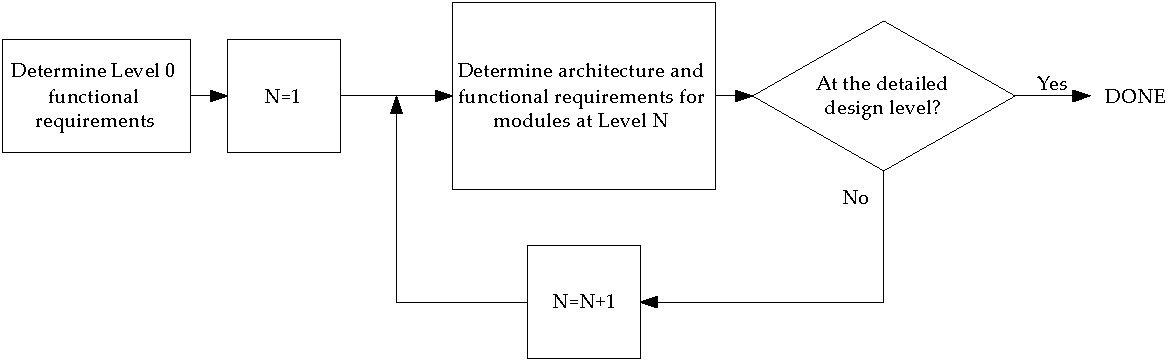
\includegraphics[width=5.5in,height=1.7in]{./image2}
\caption{A process for developing designs using functional decomposition.}
\label{figure:procFunctionalDecomposition}
\end{figure}


\section{Guidance}
\label{section:funcDecompguidance}

The following guidance is provided before examining applications of the
functional decomposition technique:

\begin{itemize}
\item
  \emph{It is an iterative process}. During the first pass, it is not
  possible to know all of the detailed interfaces between components and
  the exact functionality of each block. In fact, some details are not
  known until the implementation level is reached, so the designer needs
  to iterate, work between top-down and bottom-up, and adjust the design
  as necessary.
\item
  \emph{Set aside sufficient time to develop the design}. This is a
  corollary to the previous point. The iterative nature means that it
  takes time to examine different solutions and to refine the details
  into a working solution.
\item
  \emph{Pair together items of similar complexity.} Modules at each
  level should have similar complexity and granularity.
\item
  \emph{A good design will have the interfaces and functionality of
  modules well-defined.} It is fairly easy to piece together some blocks
  into an apparently reasonable design. However, the functional
  requirements should be clearly defined and the technical feasibility
  understood. If not, the design will fall apart when it comes to the
  implementation stage. Consider the following advice of a well-known
  architectural designer:

\begin{itquote}
The details are not the details. They make the design.---Charles Eames
\end{itquote}

\item
  \emph{Look for innovations.} Top-down designs tend to follow a
  vertical thinking process, where the designer proceeds linearly from
  problem to solution. Try to incorporate lateral thinking strategies
  from 
  Chapter~\ref{chapter:conceptGen} 
  and examine alternative architectures and technologies for the solution.
\item
  \emph{Don't take functional requirements to the absurd level.} Common
  elements, such as analog multipliers or digital logic gates, do not
  require explicit functional specifications. Doing so may become
  cumbersome and add little to the design. However, it depends upon the
  level at which you are working. If the goal is to design an analog
  multiplier chip, it is entirely appropriate to develop the functional
  requirement for the multiplier.
\item
  \emph{Combine functional decomposition with other methods of
  describing system behavior.} There is no single method or unifying
  theory for developing designs. Functional decomposition alone cannot
  describe all system behaviors. It may be supplemented by other tools
  such as flowcharts (logical behavior), state diagrams
  (stimulus-response), or data flow diagrams. In the digital stopwatch
  example presented later in this chapter, the behavior is defined using
  state diagrams. Other methods for describing system behavior are
  addressed in Chapter~\ref{chapter:behaviorModels}.
\item
  \emph{Find similar design architectures.} Determine if there exist
  similar designs and how they operate. Realize that this creates a bias
  towards existing solutions.
\item
  \emph{Use existing technology}. Many designers take the attitude that
  they are going to develop the entire design themselves, the sentiment
  being to ignore technology that they did not develop. Furthermore,
  engineering education predisposes us to design at a fundamental level.
  Both factors lead to time spent re-inventing the wheel. If existing
  technology is available that meets both the engineering and cost
  requirements, then use it.
\item
  \emph{Keep it simple}. Do not add complexity that is not needed.


\begin{itquote}
A designer knows that he has achieved perfection not when there is
nothing left to add, but when there is nothing left to take
away.---Antoine de St-Exupery
\end{itquote}


\item
  \emph{Communicate the results}. It is important to describe the theory
  of operation (the \emph{why}) as well as the implementation (the
  \emph{what}). The \emph{what} in the completed design is usually quite
  clear from the implementation, but documenting the description of
  operation and design decisions helps later when the system must
  upgraded. Designs can also become very complex, so consider how much
  information can be effectively communicated on a single page. If the
  information is too complex to show reasonably on a page or two, then
  it probably is too detailed and another level in the hierarchy should
  be added.
\end{itemize}

\section{Application: Electronics Design}
\label{section:application-electronics-design}

We now examine the application of functional decomposition in different
problem domains. In the domain of analog electronics, the inputs and
outputs of modules are voltage and current signals. Typical
transformations applied to the inputs are alterations in amplitude,
power, phase, frequency, and spectral characteristics. Consider the
design of an audio power amplifier that has the following engineering
requirements.

The system must

\begin{itemize}
\item
  Accept an audio input signal source with a maximum input voltage of
  0.5V peak.
\item
  Have adjustable volume control between zero and the maximum volume
  level.
\item
  Deliver a maximum of 50W to an 8Ω speaker.
\item
  Be powered by a standard 120V 60Hz AC outlet.
\end{itemize}

\subsection*{Level 0}
\label{subsection:level-0}
The Level 0 functionality for the amplifier is shown in 
Figure~\ref{figure:level0PowerAmp},
which is fairly simple---the inputs are an audio signal, volume control,
and wall outlet power, and the output is an amplified audio signal.

\begin{figure}[h]
\centering
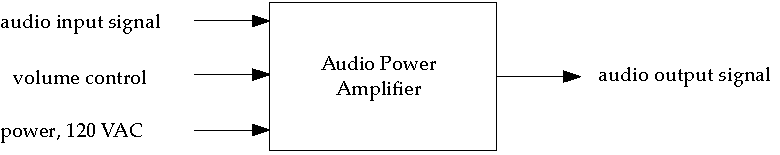
\includegraphics[width=4.1in,height=0.81in]{./image3}
\caption{Level 0 audio power amplifier functionality.}
\label{figure:level0PowerAmp}
\end{figure}

The system should be described in as much detail as possible for each
level via the functional requirement. The Level 0 functional requirement
for this design is shown in the \textbf{Audio power amplifier Module},
Table~\ref{table:functionalRequirementsAudioPowerAmplifier}.

\begin{table}[h]
\phantomcaption
\label{table:functionalRequirementsAudioPowerAmplifier}
\begin{tabular}{|l|m{10cm}|}
\hline
\emph{Module} &
Audio power amplifier \\ \hline

\emph{Inputs} & 
\begin{itemize}
\item
  Audio input signal: 0.5V peak.
\item
  Power: 120 volts AC rms, 60Hz.
\item
  User volume control: variable control.
\end{itemize} \\ \hline

\emph{Outputs} & 
\begin{itemize}
\item
  Audio output signal: \ul{?}V peak value.
\end{itemize}  \\ \hline

\emph{Functionality} & Amplify the input signal to produce a 50W maximum
output signal. The amplification should have variable user control. The
output volume should be variable between no volume and a maximum volume
level. \\ \hline
\end{tabular}
\end{table}

Not all values can be known on the first pass through the design as was
indicated in the guidelines. Underlined items represent values that need
to be determined or refined as the design proceeds. In this case, the
peak value of the audio output voltage is determined from the system
requirements on power gain. Knowing that the maximum power is given by
$P_{max} = V_{peak}^2 / R$, allows the maximum output voltage to be 
computed as  $V_{peak} = \sqrt{8\Omega*50W} = 20V$.

\subsection*{Level 1}
\label{subsection:level-1}

The Level 1 diagram, or system architecture, is shown in 
Figure~\ref{figure:level1PowerAmp}.
This architecture is common in amplifier design and is but one possible
solution. It contains three cascaded amplifier stages and a DC supply
that powers the three stages. The first amplifier stage, the
\emph{buffer amplifier}, provides a high resistance buffer that
minimizes loading effects with the source. Buffer amplifiers have
extremely high input resistance and a unity signal gain. The \emph{high
gain amplifier} increases the amplitude of the signal, but provides
little in terms of the output current necessary to drive the speakers.
The last stage in the cascade is the \emph{power output stage}, which
provides the current needed to drive the speakers, but has no voltage
amplification.

\begin{figure}[h]
\centering

\includegraphics[width=5.5in,height=2.5in]{./image6}
\caption{Level 1 audio amplifier design.}
\label{figure:level1PowerAmp}
\end{figure}

The functional requirements for the Level 1 subsystems are now detailed,
starting with the \textbf{Buffer amplifier Module},
Table~\ref{table:level1BufferAmplifier}.

\begin{table}[h]
\phantomcaption
\label{table:level1BufferAmplifier}
\begin{tabular}{|l|m{10cm}|}
\hline
\emph{Module} &
Buffer amplifier \\ \hline
\emph{Inputs} & 
\begin{itemize}
\item
  Audio input signal: 0.5V peak.
\item
  Power: ± \ul{25}V DC.
\end{itemize}\\ \hline

\emph{Outputs} & 
\begin{itemize}
\item
  Audio signal: 0.5V peak.
\end{itemize}   \\ \hline
\emph{Functionality} & Buffer the input signal and provide unity voltage
gain. It should have an input resistance \textgreater{}\ul{1M}Ω and an
output resistance \textless{}\ul{100}Ω. \\ \hline
\end{tabular}
\end{table}

Where did the ± 25V DC value for the DC input power come from? The
system must produce a ± 20V AC output signal to satisfy the Level 0
requirement, so supply values that exceed that are required to power the
electronics. How about the values for the input and output resistance?
They are educated guesses, based on knowledge of what is achievable with
the technology (bottom-up knowledge). The exact resistance requirements
are refined later based upon the overall design, taking into account the
input and output resistances for all stages.

Now consider the functional requirements shown in the 
\textbf{High gain amplifier Module}, 
Table~\ref{table:level1HighGainAmp}.

\begin{table}[h]
\phantomcaption
\label{table:level1HighGainAmp}
\begin{tabular}{|l|m{10cm}|}
\hline
\emph{Module} &
High gain amplifier \\ \hline

\emph{Inputs} & 
\begin{itemize}
\item
  Audio input signal: 0.5V peak.
\item
  User volume control: variable control.
\item
  Power: ± \ul{25}V DC
\end{itemize}\\ \hline

\emph{Outputs} & 
\begin{itemize}
\item
  Audio signal: \ul{20}V peak.
\end{itemize} \\ \hline
\emph{Functionality} & Provide an adjustable voltage gain, between \ul{1
and 40}. It should have an input resistance \textgreater{}\ul{100k}Ω and
an output resistance \textless{}\ul{100}Ω. \\ \hline
\end{tabular}
\end{table}

The gain of 40 is determined from the overall system power and gain
requirements (the maximum input voltage of 0.5V must be able to be
amplified to 20V), while the resistances are again educated guesses.

Now consider the requirements described in the 
\textbf{Power output stage Module}, 
Table~\ref{table:level1PowerOutputStage}.


\begin{table}[h]
\phantomcaption
\label{table:level1PowerOutputStage}
\begin{tabular}{|l|m{10cm}|}
\hline
\emph{Module} &
Power output stage  \\ \hline

\emph{Inputs} & 
\begin{itemize}
\item
  Audio input signal: \ul{20}V peak.
\item
  Power: ± \ul{25}V DC.
\end{itemize}\\ \hline
\emph{Outputs} & 
\begin{itemize}
\item
  Audio signal: \ul{20}V peak at up to \ul{2.5}A.
\end{itemize} \\ \hline
\emph{Functionality} & Provide unity voltage gain with output current as
required by a resistive load of up to \ul{2.5}A. It should have an input
resistance \textgreater{}\ul{1M}Ω and output resistance
\textless{}\ul{1}Ω. \\ \hline
\end{tabular}
\end{table}

For the power output stage, it is clear that 20V peak needs to be
delivered, but how was the requirement on current determined? The
current needed to drive the speaker is determined from Ohm's Law as
$I = V/R = 10V/8\Omega = 2.5A$.

The last module to examine at this level is the power supply described in
the \textbf{Power supply Module}, Table~\ref{table:level1PowerSupplyModule}.

It is clear that the power supply needs to deliver ± 25V DC, while the
3.0A current capability was selected to supply the 2.5A needed for the
peak output power requirement plus the current needed to power the other
amplifier stages.

\begin{table}[h]
\phantomcaption
\label{table:level1PowerSupplyModule}
\begin{tabular}{|l|m{10cm}|}
\hline
\emph{Module} & Power supply \\ \hline
\emph{Inputs} & 
\begin{itemize}
\item
  120 Volts AC rms.
\end{itemize} \\ \hline

\emph{Outputs} & 
\begin{itemize}
\item
  Power: ± \ul{25}V DC with up to \ul{3.0} A of current with a
  regulation of \textless{}\ul{1}\%.
\end{itemize}\\ \hline
\emph{Functionality} & Convert AC wall outlet voltage to positive and
negative DC output voltages, and provide enough current to drive all
amplifiers. \\ \hline
\end{tabular}
\end{table}

Finally, it is necessary to determine if the values of the input and
output resistances selected for the stages are realistic. For cascaded
amplifier stages, the overall voltage gain is given by the product of
gains multiplied by the voltage divider losses between stages
{[}Sed04{]}. In this case the overall gain is

$$Voltage gain = gain_1 * gain_2 * gain_3*\left[ \frac {R_{in2}} {R_{in2}+R_{out1}} \right]  * \left[ \frac{R_{in3}} {R_{in3}+R_{out2}} \right] $$
$$= 1 * 40 * 1*\left[ \frac{100k}{100k+100} \right] * \left[ \frac{1M}{1M+100} \right] = 40$$

So the resistance values selected in the functional requirements satisfy
the overall system requirements. If not, it would be necessary to go
back and refine them.

\subsection*{Level 2}
\label{subsection:level-2}

At this point, the three amplifier stages are ready for detailed
component level design, while the power supply needs another level of
refinement as shown in Figure~\ref{figure:level2PowerSupply}. 
The functional requirement for each
of the elements in the power supply would be developed similarly.
Functional decomposition stops at this point---all levels of the
hierarchy are defined and the next step is the detailed design, where
the actual circuit components are determined.

\begin{figure}[h]
\centering

\includegraphics[width=5.5in,height=0.85in]{./image9}
\caption{Level 2 design of the power supply.}
\label{figure:level2PowerSupply}
\end{figure}

\section{Application: Digital Design}
\label{section:application-digital-design}

Functional decomposition is widely applied to the design of digital
systems, where it is known as \emph{entity-architecture} design. The
inputs and outputs refer to the entity, and the architecture describes
the functionality. The application of functional decomposition to
digital systems is demonstrated in the following example. Consider the
design of a simple digital stopwatch that keeps track of seconds and has
the following engineering requirements.

The system must

\begin{itemize}
\item  Have no more than two control buttons.
\item  Implement Run, Stop, and Reset functions.
\item  Output a 16-bit binary number that represents seconds elapsed.
\end{itemize}

\subsection*{Level 0}
\label{subsection:level-0-1}


The Level 0 diagram and functional requirements are shown in
Figure~\ref{figure:level0Stopwatch}.

\begin{figure}[h]
\centering
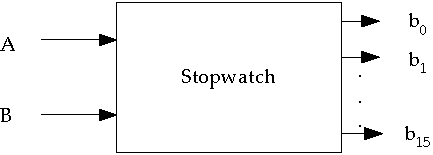
\includegraphics[width=2.7in,height=0.96in]{./image10}
\caption{Level 0 digital stopwatch functionality.}
\label{figure:level0Stopwatch}
\end{figure}

The Level 0 functional requirement
for this design is shown in the \textbf{Stopwatch Module},
Table~\ref{table:level0StopWatch}.


\begin{table}[h]
\phantomcaption
\label{table:level0StopWatch}
\begin{tabular}{|l|m{10cm}|}
\hline
\emph{Module} & Stopwatch \\ \hline
\emph{Inputs} & 
\begin{itemize}
\item
  A: Reset button signal. When the button is pushed it resets the
  counter to zero.
\item
  B: Run/stop toggle signal. When the button is pushed it toggles
  between run and stop modes.
\end{itemize}\\ \hline

\emph{Outputs} & 
\begin{itemize}
\item
  b\textsubscript{15}-b\textsubscript{0}: 16-bit binary number that
  represents the number of seconds elapsed.
\end{itemize} \\ \hline
\emph{Functionality} & The stopwatch counts the number of seconds after
B is pushed when the system is in the Reset or Stop mode. When in Run
mode and B is pushed, the stopwatch stops counting. A reset button push
(A) will reset the output value of the counter to zero only when in Stop
mode. \\ \hline
\end{tabular}
\end{table}

\subsection*{Level 1}
\label{subsection:level-1-1}
The Level 1 architecture in Figure~\ref{figure:level1Stopwatch}
contains three modules: a seconds
counter, a clock divider, and a finite state machine (FSM). The
stopwatch counts seconds, thus the seconds counter module counts the
seconds and outputs a 16-bit number representing the number of seconds
elapsed. The clock divider generates a 1Hz signal that triggers the
seconds counter. The FSM responds to the button press stimuli and
produces the appropriate control signals for the seconds counter. The
system clock is included to clock both the FSM and the clock divider.

\begin{figure}[h]
\centering
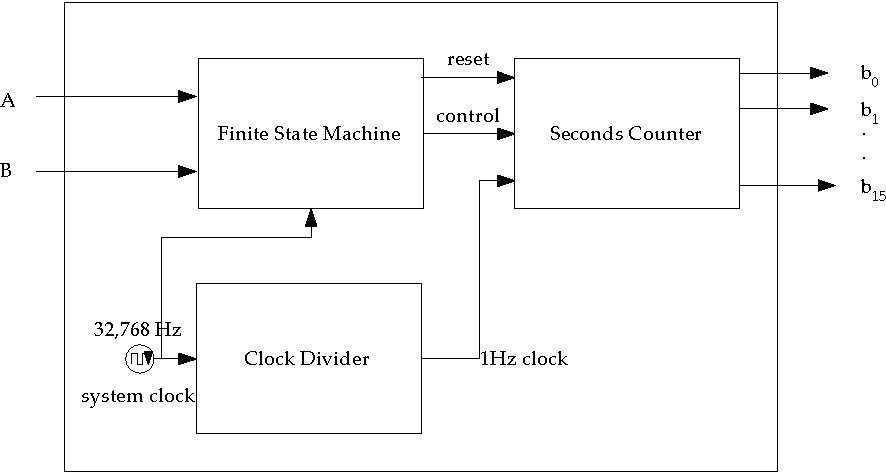
\includegraphics[width=5.5in,height=2.95in]{./image11}
\caption{Level 1 design for the digital stopwatch..}
\label{figure:level1Stopwatch}
\end{figure}

The functionality of the Level 1 modules is described as follows,
starting with 
the \textbf{Finite state machine Module}, Table~\ref{table:level1FiniteStateMachine}.

\begin{table}[h]
\phantomcaption
\label{table:level1FiniteStateMachine}
\begin{tabular}{|l|m{10cm}|}
\hline
\emph{Module} & Finite State Machine \\ \hline
\emph{Inputs} & 
\begin{itemize}
\item
  A: Signal to reset the counter.
\item
  B: Signal to toggle the stopwatch between run and stop modes.
\item
  Clock: 1Hz clock signal.
\end{itemize}\\ \hline

\emph{Outputs} & 
\begin{itemize}
\item
  Reset: Signal to reset the counter to zero.
\item
  Control: Signal that enables or disables the counter.
\end{itemize} \\ \hline
\emph{Functionality} &

\includegraphics[width=2in,height=1.2in]{./image12} \\ \hline
\end{tabular}
\end{table}

The functionality of the finite state machine is described with a tool
that is probably familiar to the reader, the state diagram. State
diagrams are covered in more detail in
 Chapter~\ref{chapter:behaviorModels}. The state diagram
describes stimulus-response behavior, and shows how the system
transitions between states based upon logic signals from the button
presses.

Next, consider 
the \textbf{Clock divider Module}, Table~\ref{table:stopwatchClockDivider}.

\begin{table}[h]
\phantomcaption
\label{table:stopwatchClockDivider}
\begin{tabular}{|l|m{10cm}|}
\hline
\emph{Module} & Clock Divider\\ \hline
\emph{Inputs} & 
\begin{itemize}
\item
  System clock: \ul{32,768}Hz.
\end{itemize}\\ \hline

\emph{Outputs} & 
\begin{itemize}
\item
  Internal clock: 1Hz clock for seconds elapsed.
\end{itemize} \\ \hline
\emph{Functionality} & Divide the system clock by 32,768 to produce a
1Hz clock. \\ \hline
\end{tabular}
\end{table}

The value of 32,768 Hz was selected for the system clock for several
reasons. It is a power of 2 that is easily divisible by digital
circuitry to produce a 1Hz output signal. It is also well above the
clock rate needed for detecting button presses and there is a wide
selection of crystals that can meet this requirement.

Finally, consider 
the \textbf{Second counter Module}, Table~\ref{table:level1stopwatchSecondsCounter}.

\begin{table}[h]
\phantomcaption
\label{table:level1stopwatchSecondsCounter}
\begin{tabular}{|l|m{10cm}|}
\hline
\emph{Module} & Seconds counter\\ \hline
\emph{Inputs} & 
\begin{itemize}
\item
  Reset: Reset the counter to zero.
\item
  Control: Enable/disable the counter.
\item
  Clock: Increment the counter.
\end{itemize}\\ \hline

\emph{Outputs} & 
\begin{itemize}
\item
  b\textsubscript{15}-b\textsubscript{0}: 16-bit binary representation
  of number of seconds elapsed.
\end{itemize}\\ \hline
\emph{Functionality} & Count the seconds when enabled and resets to zero
when reset signal enabled. \\ \hline
\end{tabular}
\end{table}



The system decomposition would end here, assuming that the design is to
be implemented using off-the-shelf chips. The next step would be to
determine components at the detailed design level. However, if it were
an integrated circuit design, the description would continue until the
transistor level is reached.

\section{Application: Software Design}
\label{section:application-software-design}

Software also lends itself to functional decomposition since virtually
all computing languages provide the capability to call functions,
subroutines, or modules. Functional software design simplifies program
development by eliminating the need to create redundant code via the use
of functions that are called repeatedly.

\emph{\textbf{Structure charts}} are specialized block diagrams for
visualizing functional software designs. The modules used in a structure
chart are shown in 
Figure~\ref{figure:softwareModules}. The larger arrows indicate connections to
other modules, while the smaller arrows represent data and control
information passed between modules. Five basic modules are utilized:

\begin{enumerate}
\def\labelenumi{\arabic{enumi}.}
\item
  \emph{Input} \emph{modules}. Receive information.
\item
  \emph{Output} \emph{modules.} Return information.
\item
  \emph{Transform} \emph{modules.} Receive information, change it, and
  return the changed information.
\item
  \emph{Coordination} \emph{modules.} Coordinate or synchronize
  activities between modules.
\item
  \emph{Composite} \emph{modules.} Any possible combination of the other
  four.
\end{enumerate}

This approach to software design, also known as \emph{structured
design}, was formalized in the 1970's by IBM researchers {[}Ste99{]}.

\begin{figure}[h]
\centering

\includegraphics[width=5.5in,height=1.4in]{./image13}
\caption{Module types for functional software design. The
larger arrows indicate connections between modules and the smaller
arrows represent data and control.}
\label{figure:softwareModules}
\end{figure}

The following example demonstrates the application of functional
decomposition to a software design with the following requirements.

The system must

\begin{itemize}
\item
  Accept an ASCII file of integer numbers as input.
\item
  Sort the numbers into ascending order and save the sorted numbers to
  disk.
\item
  Compute the mean of the numbers.
\item
  Display the mean on the screen.
\end{itemize}

This is a fairly simple task that could easily be done in a single
function, but doing so would not allow components of the design to be
easily reused, tested, or troubleshot. The engineering requirements
themselves provide some guidance in terms of how to arrange the
functionality of the modules (\emph{form follows function}). The
architecture in 
Figure~\ref{figure:structureChartSorting} contains a main module that calls three
sub-modules. In this design main is a coordinating module that controls
the processing and calling of the other modules, a common scenario. It
was also decided that all user interaction would take place within main.
The order of the processing is not described by structure charts. In our
program, main calls ReadArray, SortArray, and ComputeMean in sequential
order. main passes the filename (fname) to ReadArray, which reads in the
array and the number of elements in it, and returns this information to
main. The choice of passing in the filename was deliberate; the user
could have been prompted for the filename in ReadArray, but doing so
might limit future reuse of the function since you may not always want
to do so when reading an array of data. SortArray is then called, which
accepts the array of numbers and the number of elements in the array,
and returns the sorted values in the same array. Finally, ComputeMean is
executed, which accepts the sorted array and the number of elements,
computes the mean value, and returns it to main.

\begin{figure}[h]
\centering
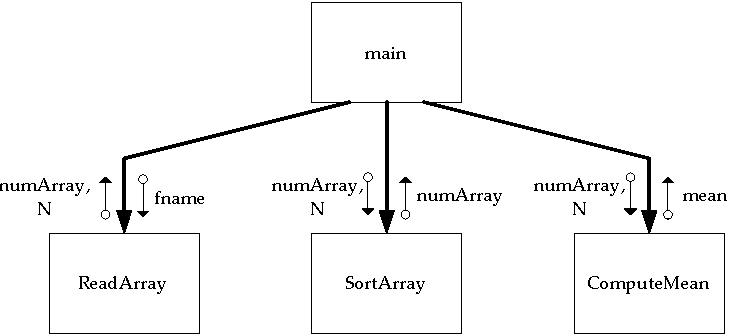
\includegraphics[width=4.1in,height=1.9in]{./image14}
\caption{Structure chart design of sorting and mean
computation program.}
\label{figure:structureChartSorting}
\end{figure}


The functional requirements for each module in the structure chart are
detailed in Table~\ref{table:functionalSort}. 
The structure chart provides a visual
relationship between modules in the design, but also has some
disadvantages. It is difficult to visualize designs as the complexity of
the software increases. This can be addressed by expanding sublevels in
the design as necessary in different diagrams. Structure charts also
lack a temporal aspect that indicates the calling order. Most software
systems have many layers in the hierarchy and highly complex calling
patterns. In this example, main calls three modules in a well-defined
order, but if there was another level in the hierarchy, there is no
reason why it could not be called by a module at any other level. That
leads to some of the unique problems associated with software design.
Functional design works well for small-to-moderately complex software,
but tends to fall short when applied to large scale software systems. As
such, it has given way to the object-oriented design approach.

\section{Application: Thermometer Design}
\label{section:application-thermometer-design}

The final example includes both analog and digital modules where the
objective is to design a thermometer that meets the following
engineering requirements.

The system must

\begin{itemize}
\item  Measure temperature between 0 and 200$^\circ$C.
\item  Have an accuracy of 0.4\% of full scale.
\item  Display the temperature digitally, including one digit beyond the
  decimal point.
\item  Be powered by a standard 120V 60Hz AC outlet.
\item  Use an RTD (thermal resistive device) that has an accuracy of 0.55$^\circ$C
  over the range. The resistance of the RTD varies linearly with
  temperature from 100$\omega$ at 0$^\circ$C to 178$\omega$ at 200$^\circ$C. (Note: this requirement
  does not meet the abstractness property identified in 
  Chapter~\ref{chapter:requirementSpec}, since
  it identifies part of the solution. This requirement is given to
  provide guidance in this example.)
\end{itemize}



\begin{table}[h]
\small
\caption{Functional design requirements for the number  sort  program.}
\label{table:functionalSort}

\begin{tabular}{|l|m{10cm}|}
\hline
\emph{Module name} & main\\ \hline
\emph{Module type} & Coordination \\ \hline
\emph{Input arguments} & None \\ \hline
\emph{Output arguments} & None \\ \hline
\emph{Description} & The main function calls ReadArray() to read the
input file from disk, SortArray() to sort the array, and ComputeMean()
to determine the mean value of elements in the array. User interaction
requires the user to enter the filename, and the mean value is displayed
on the screen. \\ \hline
\emph{Modules invoked} & ReadArray, SortArray, and ComputeMean \\ \hline
\end{tabular}
\vspace{0.2cm}

\begin{tabular}{|l|m{10cm}|}
\hline
\emph{Module name} & ReadArray() \\ \hline
\emph{Module type} & Input and output \\ \hline
\emph{Input arguments} & 
\begin{itemize}
\item fname{[}{]}: character array with filename to read from.
\end{itemize} \\ \hline
\emph{Output Arguments} & 
\begin{itemize}
\item numArray{[}{]}: integer array with elements read from file.
\item  N: number of elements in numArray{[}{]}.
\end{itemize}\\ \hline
\emph{Description} & Read data from input data file and store elements
in array numArray{[}{]}. The number of elements read is placed in N. \\ \hline
\emph{Modules invoked} & None \\ \hline
\end{tabular}
\vspace{0.2cm}

\begin{tabular}{|l|m{10cm}|}
\hline
\emph{Module name} & SortArray() \\ \hline
\emph{Module type} & Transformation \\ \hline
\emph{Input arguments} & 
\begin{itemize}
\item   numArray{[}{]}: integer array of numbers.
\item   N: number of elements in numArray{[}{]}.
\end{itemize}  \\ \hline
\emph{Output Arguments} & 
\begin{itemize}
\item  numArray{[}{]}: sorted array of integer numbers.
\end{itemize} \\ \hline
\emph{Description} & Sort elements in array using a shell sort
algorithm. Saves the the sorted array to disk. \\ \hline
\emph{Modules invoked} & None \\ \hline
\end{tabular}
\vspace{0.2cm}

\begin{tabular}{|l|m{10cm}|}
\hline
\emph{Module name} & ComputeMean()\\ \hline
\emph{Module type} & Input and output \\ \hline
\emph{Input arguments} & 
\begin{itemize}
\item  numArray{[}{]}: integer array of numbers.
\item  N: number of elements in numArray{[}{]}.
\end{itemize} \\ \hline
\emph{Output arguments} & 
\begin{itemize}
\item  mean: mean value of the elements in the array.
\end{itemize} \\ \hline
\emph{Description} & Computes the mean value of the integer elements in
the array. \\ \hline
\emph{Modules invoked} & None \\ \hline
\end{tabular}

\end{table}



\subsection*{Level 0}
\label{subsection:level-0-2}

The overall goal is to convert a sensed temperature to a digital
temperature reading. The Level 0 description description is 
shown in Figure~\ref{figure:digitalTermLevel0}.

\begin{figure}[h]
\centering
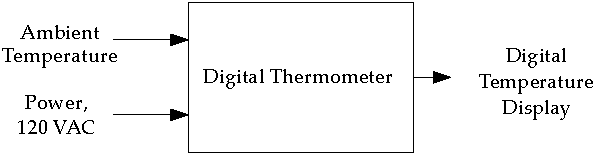
\includegraphics[width=3.4in,height=0.88in]{./image15}
\caption{Level 0 digital thermometer functionality.}
\label{figure:digitalTermLevel0}
\end{figure}


The input, output and functioality of the signal in Figure~\ref{figure:digitalTermLevel0} are
described in the \textbf{Digital thermometer Module}, Table~\ref{table:digitalThermLevel0}.

\begin{table}[h]
\phantomcaption
\label{table:digitalThermLevel0}
\begin{tabular}{|l|m{10cm}|}
\hline
\emph{Module name} & Digital Thermometer \\ \hline
\emph{Inputs} & 
\begin{itemize}
\item Ambient temperature: 0-200°C.
\item Power: 120V AC power.
\end{itemize}  \\ \hline
\emph{Outputs} & 
\begin{itemize}
\item
  Digital temperature display: A four digit display, including one digit
  beyond the decimal point.
\end{itemize} \\ \hline
\emph{Functionality} & Displays temperature on digital readout with an
accuracy of 0.4\% of full scale. \\ \hline
\end{tabular}
\end{table}

\subsection*{Level 1}
\label{subsection:level-1-2}

The Level 1 architecture selected is shown in 
Figure~\ref{figure:level1DigitalThermo}. The
temperature conversion unit converts the temperature to an analog
voltage using the RTD that is sampled by the analog-to-digital
converter. The N-bit binary output from the converter is translated into
binary-coded decimal (BCD). BCD is a 4-bit representation of the digits
between 0 and 9. Since there are four display digits, there are four
separate binary encoded outputs from the BCD conversion unit. Common
7-segment LEDs are used for the display. However, they do not directly
accept BCD and instead have seven input lines, each of which is
individually switched to control the display segments. The requirements
did not specifically address cost or size constraints, nor clearly
define the environment, so there are many possible solutions. For
example, an analog-to-digital current converter could be used,
integrated circuit temperature sensing packages could be considered, and
microcontroller-based solutions are feasible as well.

From a system design perspective, an error budget is needed to identify
the maximum error that each subsystem may introduce, while still
achieving the overall accuracy. In this case, error is introduced in the
temperature conversion unit and A/D converter, but not in the remaining
digital components. The overall accuracy that the system must achieve is
0.4\%, and that translates into 0.8°C of allowable error for the 200°C
range. Let's now examine the modules.

\begin{figure}[h]
\centering
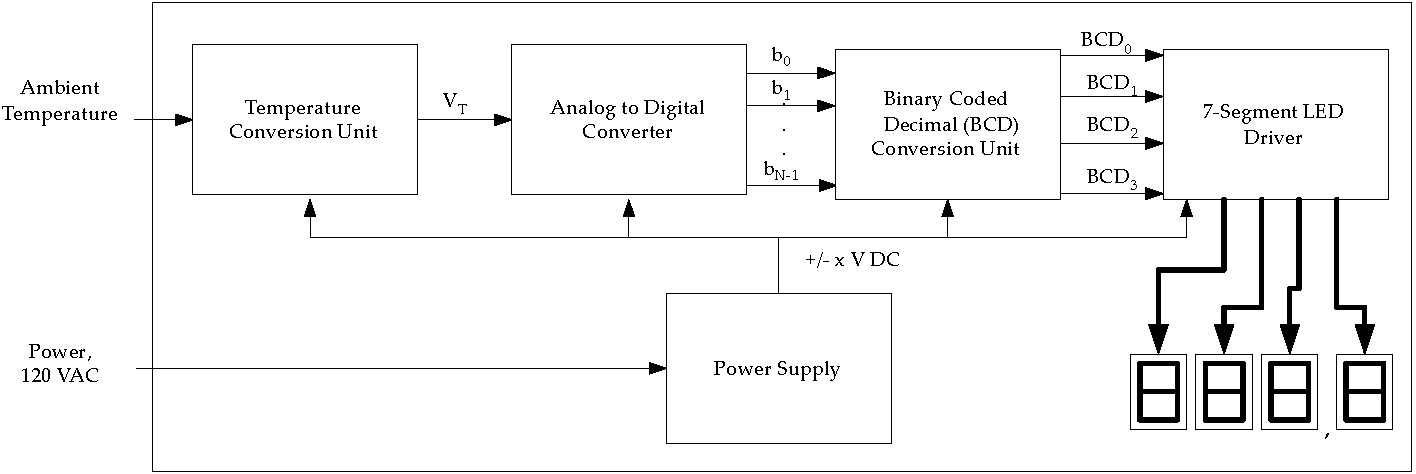
\includegraphics[width=5.5in,height=1.8in]{./image16}
\caption{Level 1 design of the digital thermometer.}
\label{figure:level1DigitalThermo}
\end{figure}

The functionality of the Level 1 modules is described as follows,
starting with the temperature conversion unit.
the \textbf{Temperature conversion unit supply Module}, 
Table~\ref{table:digitalThermoTempConvUnit}.


\begin{table}[h]
\phantomcaption
\label{table:digitalThermoTempConvUnit}
\begin{tabular}{|l|m{10cm}|}
\hline
\emph{Module} & Temperature conversion unit\\ \hline
\emph{Inputs} & 
\begin{itemize}
\item  Ambient temperature: 0-200°C.
\item  Power: \ul{?}V DC (to power the electronics).
\end{itemize}  \\ \hline
\emph{Outputs} & 
\begin{itemize}
\item  V\textsubscript{T}: temperature proportional voltage.
  V\textsubscript{T}= \underline{$\alpha$}T, and ranges from \underline{?} to \underline{?}V.
\end{itemize}\\ \hline
\emph{Functionality} & Produces an output voltage that is linearly
proportional to temperature. It must achieve an accuracy of \underline{?}\%. \\ \hline
\end{tabular}
\end{table}

There are several unknowns at this point. The voltage necessary to power
the electronics is not known, but a reasonable assumption could be made.
The output voltage range and the accuracy are unknown. It is known that
the RTD will introduce up to 0.55°C of error and that the electronics
themselves will introduce additional error (the exact amount is unknown
at this point). An educated guess is made that the maximum error allowed
for the temperature unit is 0.6°C. This means that the electronics
themselves would be required to introduce no more than 0.05°C of error
due to the 0.55°C of error introduced by the RTD.

Now consider the 
the \textbf{A/D converter Module}, 
Table~\ref{table:digitalThermoDigitalConverter}.


\begin{table}[h]
\phantomcaption
\label{table:digitalThermoDigitalConverter}
\begin{tabular}{|l|m{10cm}|}
\hline
\emph{Module} & A/D converter\\ \hline
\emph{Inputs} & 
\begin{itemize}
\item
  V\textsubscript{T}: voltage proportional to temperature that ranges
  from \ul{?} to \ul{?}V.
\item  Power: \ul{?}V DC.
\end{itemize}  \\ \hline
\emph{Outputs} & 
\begin{itemize}
\item  b\textsubscript{N-1} -b\textsubscript{0}: \ul{?-}bit binary
  representation of V\textsubscript{T}.
\end{itemize}\\ \hline
\emph{Functionality} & Converts analog input to binary digital
output. \\ \hline
\end{tabular}
\end{table}



The A/D converter is not likely to be something that is designed due to
the availability of low cost, off-the-shelf solutions. The requirements
drive the converter selection. There are two unknowns\emph{---}the
number of bits and the range of the input voltage. The number of bits
affects the accuracy, since the greater the number of bits, the better
the accuracy. The number of bits needed for the converter is calculated
from the maximum allowable error that the A/D can introduce (0.2°C), the
number of discrete intervals, and the temperate range as

$$Max error = \frac{range}{number of intervals} = \frac{200^{\circ}  C}{2^N} \leq 0.2^{\circ}  C \Rightarrow N \geq 9.97 bits$$

So the A/D converter needs to have at least 10 bits. How is the voltage
range selected? It is typically fixed for a particular integrated
circuit solution, but the temperature conversion subsystem output should
be matched to the voltage range so that all bits are effectively
utilized, otherwise, error is introduced.

Now, consider 
the \textbf{BCD conversion unit Module}, 
Table~\ref{table:digitalThermoBcdConvUnit}.


\begin{table}[h]
\phantomcaption
\label{table:digitalThermoBcdConvUnit}
\begin{tabular}{|l|m{10cm}|}
\hline
\emph{Module} & BCD conversion unit\\ \hline
\emph{Inputs} & 
\begin{itemize}
\item
  10-bit binary number (b\textsubscript{9}-b\textsubscript{0}):
  Represents the range 0.0-200.0°C.
\item
  Power: \ul{?}V DC.
\end{itemize}  \\ \hline
\emph{Outputs} & 
\begin{itemize}
\item
  BCD\textsubscript{0}: 4-bit BCD representation of tenths digit (after
  decimal).
\item
  BCD\textsubscript{1}: 4-bit BCD representation of one's digit.
\item
  BCD\textsubscript{2}: 4-bit BCD representation of ten's digit.
\item
  BCD\textsubscript{3}: 4-bit BCD representation of hundred's digit.
\end{itemize}\\ \hline
\emph{Functionality} & Converts the 10-bit binary number to BCD
representation of temperature. Must refresh the displays twice a
second. \\ \hline
\end{tabular}
\end{table}



The objective of the BCD conversion unit is fairly simple, although the
component level design of the circuitry to accomplish the conversion is
not.

This leads to the last module, 
the \textbf{7-Segment LED driver Module}, 
Table~\ref{table:digitalThermoSevenSeg}.


\begin{table}[h]
\phantomcaption
\label{table:digitalThermoSevenSeg}
\begin{tabular}{|l|m{10cm}|}
\hline
\emph{Module} & 7-Segment LED driver\\ \hline
\emph{Inputs} & 
\begin{itemize}
\item
  BCD\textsubscript{0}: 4-bit BCD representation of tenths digit (after
  decimal).
\item
  BCD\textsubscript{1}: 4-bit BCD representation of one's digit.
\item
  BCD\textsubscript{2}: 4-bit BCD representation of ten's digit.
\item
  BCD\textsubscript{3}: 4-bit BCD representation of hundred's digit.
\item
  Power: \ul{?}V DC.
\end{itemize}  \\ \hline
\emph{Outputs} & 
\begin{itemize}
\item
  Four 7-segment driver lines.
\end{itemize}\\ \hline
\emph{Functionality} & Converts the BCD for each digit into outputs that
turn on LEDs in 7-segment package to display the temperature.  \\ \hline
\end{tabular}
\end{table}



For completeness, the functional requirements of
the \textbf{Power supply Module}, 
Table~\ref{table:digitalThermoPowerSupply} are supplied. 
They are similar to the power supply requirements utilized in
the audio amplifier design in Section~\ref{section:application-electronics-design}.


\begin{table}[h]
\phantomcaption
\label{table:digitalThermoPowerSupply}
\begin{tabular}{|l|m{10cm}|}
\hline
\emph{Module} & Power supply\\ \hline

\emph{Inputs} & 
\begin{itemize}
\item  120 Volts AC rms.
\end{itemize} \\ \hline

\emph{Outputs} & 
\begin{itemize}
\item  ± \ul{?}V DC with up to \ul{?}mA of current.
\item  Regulation of \ul{?}\%.
\end{itemize}\\ \hline

\emph{Functionality} & Convert AC wall outlet voltage to positive and
negative DC output voltages, with enough current to drive all circuit
subsystems. \\ \hline

\end{tabular}
\end{table}



At this point, the requirements for the major subsystems are completed
and ready for design at the component level. Illustration of the
complete design would require a fair amount of detail, and while it is
not presented here, some of the issues involved are discussed. First,
there are a variety of electronic circuits (inverting op amps, single
BJT configurations, and current mirrors, etc.---see 
Section~\ref{subsection:analytical-hierarchy-process-and-decision-matrices} ) 
that could be utilized as a current source to drive the RTD
in the temperature conversion subsystem. A midrange resolution A/D
converter is needed, and its particular input voltage range drives the
output voltage requirements for the temperature conversion module. The
BCD conversion circuitry could be implemented using combinational
digital logic (tedious due to the number of discrete gates), or a more
efficient, but slower, sequential logic design. Finally, the 7-segment
display converters could be designed using combinational logic that maps
the BCD inputs into outputs to activate the appropriate display
segments.

\section{Coupling and Cohesion}
\label{section:coupling-and-cohesion}

The concepts of coupling and cohesion are examined before concluding
this chapter. They originated to describe software designs {[}Ste99{]},
but are applicable to electrical and computer systems. To understand
their importance, consider the relationship between the number of
modules in a system and the number of connections between them. For our
purposes, a connection between two modules may consist of any number of
signals without regard to their direction. Thus, a system consisting of
two modules has, at most, one connection. If the number of modules is
increased to three, the number of possible connections increases to
three, a system with four modules has six possible connections, and five
modules increases the number of possible connections to ten. The point
is that the maximum number of potential connections increases rapidly
with the number of modules in the system. The relationship between the
maximum possible connections and number of modules (\emph{n}) is given
by
$$Connections_{max} = \frac{n(n-1)}{2}$$

Modules are coupled if they depend upon each other in some way to
operate properly. \emph{\textbf{Coupling}} is the extent to which
modules or subsystems are connected {[}Jal97{]}. Although there is no
agreed upon mathematical definition of coupling, it seems obvious that
increasing the exchange of control and data between two modules leads to
a higher degree of coupling. When systems are highly coupled, it is
difficult to change one module without impacting the other. Consider the
extreme case where all modules in a system are connected to each
other---an error in one module has the potential to impact every other
module in the system. Errors in a module are propagated to others to a
degree that is related to the amount of coupling. From this point of
view, it is good to minimize coupling. Yet coupling cannot be
eliminated, since the point of functional decomposition is to break a
design into components that work together to produce a higher level
behavior.

There are two ways to reduce coupling---minimize the number of
connections between modules and maximize cohesion within modules.
\emph{\textbf{Cohesion}} refers to how focused a module is---highly
cohesive systems do one or a few things very well. Stevens \emph{et al.}
{[}Ste99{]} defined six types of cohesion from the weakest to strongest
as: coincidental, logical, temporal, communicational, sequential, and
functional. More information on this can be found in the original work,
but the conclusion is that modules with high functional cohesion are the
most desirable. So it is best to design modules with a single
well-defined functional objective consistent with the philosophy of
functional decomposition. This leads to the important design principle
that it is desirable to maximize cohesion, while minimizing coupling.

Coupling and cohesion impact the later stages of testing and system
integration. If a particular module is highly cohesive, then it should
be possible to test it independently of the other modules to verify its
operability. This does not mean that it will necessarily operate
properly when integrated into the overall system, but the probability
that it will is higher if provided with proper inputs from connected
modules. Contrast this to the case of a low cohesion system. In that
case, it will likely be difficult to test the individual modules without
first integrating them.

To develop a better understanding, consider the amplifier design in
Figure~\ref{figure:level1PowerAmp}
(Section~\ref{section:application-electronics-design}) 
with three cascaded amplifier stages. Each
stage is highly cohesive, performing a singular function of signal
amplification. Each of these stages could easily operate as a
stand-alone module independent of the complete system. How about
coupling? In terms of the number of connections, it is fairly low as
each amplifier stage has an input and output voltage signal. The most
coupled module in the system is the power supply, and not surprisingly,
its failure leads to a complete system failure. Coupling in this case
can also be viewed in terms of the resistance matching between input and
output of the cascaded stages, producing the voltage divider effect in
equation (1). For voltage amplifiers, the goal is to have high input
resistance and low output resistance, which minimize both voltage losses
and coupling. The stages are not completely uncoupled, because the input
resistances, although large, are not infinite, and the output
resistances are not zero. The modules in the power supply unit in 
Figure~\ref{figure:level2PowerSupply}
(rectifier, smoothing filter, and regulator) have a much higher
degree of coupling. In fact, it is difficult to develop a clear
functional decomposition of the power supply module because the elements
in the smoothing filter also serve as part of the rectifier circuit
(refer to a basic electronics textbook {[}Sed04{]} for more
information).

As another example, consider a software design where two options are
under consideration: one large function with 1000 lines of code, versus
15 cohesive functions, each with an average of 100 lines of code. Both
perform the same function, but which runs faster? Most likely the first,
as it would be highly integrated and would not suffer from overhead
needed with multiple functions. Which is easier to upgrade and debug a
year from now? That is clearly the second case. Although loosely coupled
and highly cohesive designs may facilitate better design and testing,
they may not be best in terms of performance.

\section{Project Application: The Functional Design}
\label{section:project-application-the-functional-design}

The following is a format for documenting and presenting functional
designs.


\textbf{Design Level 0}
\begin{itemize}
\item  Present a single module block diagram with inputs and outputs
  identified.
\item  Present the functional requirements: inputs, outputs, and
  functionality.
\end{itemize}


\textbf{Design Level 1}
\begin{itemize}
\item
  Present the Level 1 diagram (system architecture) with all modules and
  interconnections shown.
\item
  Describe the theory of operation. This should explain how the modules
  work together to achieve the functional objectives.
\item
  Present the functional requirements for each module at this level.
\end{itemize}


\textbf{Design Level N (for N\textgreater1)}
\begin{itemize}
\item
  Repeat the process from Design Level 1 for as many levels as
  necessary.
\end{itemize}

\textbf{Design Alternatives}
\begin{itemize}
\item
  Describe the different alternatives that were considered, the
  tradeoffs, and the rationale for the choices made. This should be
  based upon concept evaluation methods communicated in 
  Chapter~\ref{chapter:conceptGen}.
\end{itemize}

\section{Summary and Further Reading}
\label{section:funcDecomSummary-and-further-reading}

This chapter presented the functional decomposition design technique,
where every level of the design is decomposed into sub-modules, each of
which is the domain of the next lower level. The inputs, outputs, and
functionality must be determined for a given module. Applying the
process in Figure~\ref{figure:procFunctionalDecomposition}
and following the guidelines in Section~\ref{section:funcDecompguidance} should
aid in the application of functional decomposition. Functional
decomposition is applicable to a wide variety of systems, and in this
chapter designs of analog electronics, digital electronics, and software
were examined.

Nigel Cross presents a good overview of the functional decomposition
method with application to mechanical systems {[}Cro00{]}, but with less
focus on the description of the functional requirements than presented
here. The work by Stevens \emph{et al}. {[}Ste99{]} is interesting
reading that gives an understanding of the evolution of structured
design. It delves into the concepts of coupling and cohesion. Coupling
and cohesion are also addressed well in the book by Jalote {[}Jal97{]}.
An in-depth treatment of structured systems design is found in \ul{The
Practical Guide to Structured Systems Design} {[}Pag88{]}. This guide
also integrates data flow diagrams with functional techniques. Finally,
the thermometer design example was inspired by Stadtmiller's book
{[}Sta01{]} on electronics design.
